

%\documentstyle[12pt]{article}
\documentclass[12pt]{article}
\setlength{\oddsidemargin}{0in}
\setlength{\evensidemargin}{0in}
\setlength{\textwidth}{6.5in}
\setlength{\topmargin}{-0.3in}
\setlength{\textheight}{9in}
\pagestyle{empty}
\usepackage{natbib}
\usepackage{amsmath}
\usepackage{graphicx}
\usepackage{caption}
\usepackage{subcaption}

\newcommand\tab[1][3cm]{\hspace*{#1}}

\begin{document}

\begin{center}
{\Large \textbf{Out of Distribution Detection Using Bayesian Variational Autoencoder}} \\[.2in]
{\large Kamran Chitsaz   \tab   Alireza Razaghi}
\end{center}

\vspace*{.05in}


\section{Introduction}

The recent success of deep learning methods plays an essential role in the evolution at an unprecedented rate of current technology. Despite their remarkable performance in a wide range of complex tasks including image recognition \cite{krizhevsky2012imagenet}, object detection \cite{girshick2014rich}, and speech recognition \cite{deng2013recent}, deep learning models can make confident, but meaningless, predictions on unobserved data \cite{nguyen2015deep}. To perform reliable decisions, Deep learning models need to be able to determine whether the input data is an anomaly or outlier and significantly different from the training data. Such data are called out-of-distribution (OoD) data. Several approaches have been proposed to detect OoD data such as spectral anomaly detection techniques which try to find lower dimensional embeddings of the input data where OoD and normal data are expected to be separated from each other. The Principal components analysis (PCA) \cite{chandola2009anomaly} and Autoencoders \cite{sakurada2014anomaly} are among the most popular dimension reduction methods for detecting outliers.


Likelihood estimators are one of the most promising OoD detection approach which work for probabilistic generative models. Such models can evaluate the likelihood of input data, and if a generative model fits the training data distribution well enough, it should assign high likelihood to samples from the similar distribution and low likelihood to OoD samples. So to detect whether a data is OoD or not, by this approach first trains a density estimator parameterized by $\theta$, and then classifies an input $\mathbf{x}^{*}$ as OoD based on a threshold on the density of $\mathbf{x}^{*}$, i.e., if $p\left(\mathbf{x}^{*} \mid \theta\right)<\tau$ \cite{bishop1994novelty}. In this project we used variational autoencoder to calculate log likelihood and detect OoD.


\section{Background}

One of the most popular models for density estimation is the Variational Autoencoder \cite{kingma2013auto} which successfully can approximate the distribution of training data. By this generative model we can learn a joint model $p(x,z)$ of the data $x$ and some latent variables $z$. The idea is that each data X has a corresponding latent variable Z that data X is caused by this Z, so we can marginalize out Z. 
$$p(x)=\int p(x | z) p(z) dz$$
The conditional distribution $p(x | z)$ is a Gaussian. So, we have a kind of mixture of infinitely many Gaussians, for each value of Z, there's one Gaussian and we mix them with weights. In this approach we assumed that prior is normal and likelihood is a Gaussian which it's parameters are depend on latent variable z. One way to define parameters is using neural networks. So the parameters of our model depends on leading variable z which is generated by a neural network with parameter $\theta$. So we can build the observation model as follow:
$$\begin{array}{l}
p(x)=\int p(x | z) p(z) dz \\
p(z)=\mathcal{N}(0, I) \\
p(x \mid z)=\mathcal{N}\left(x \mid \mu_{\theta}(z), diag\left(\sigma_{\theta}^{2}(z)\right)\right)
\end{array}$$


Since computing $p_{\theta}(\mathbf{x})=\int p_{\theta}(\mathbf{x} \mid \mathbf{z}) p(\mathbf{z}) \mathrm{d} \mathbf{z}$ is intractable in high dimention, variational inference is used to derive a lower bound on the log likelihood of x. So we can approximate posterior $p_{\theta}(\mathbf{z} \mid \mathbf{x})$ using amortized variational inference via another neural network with parameter $\phi$. Similarly, we can build the inference model as
$$
q(z \mid x)=\mathcal{N}\left(z \mid \mu_{\phi}(x), \operatorname{diag}\left(\sigma_{\phi}^{2}(x)\right)\right)
$$
Using Jensen’s inequality we have

$$
\begin{aligned}
\log p(x)=& \log \int \frac{q(z \mid x)}{q(z \mid x)} p(x, z) d z  \geq \int q(z \mid x) \log \frac{p(x, z)}{q(z \mid x)} d z \\
&=\mathbb{E}_{q(z \mid x)} \log \frac{p(x, z)}{q(z \mid x)} =\mathbb{E}_{q(z \mid x)} \log \frac{p(x \mid z) p(z)}{q(z \mid x)}
\end{aligned}
$$
%= \mathcal{L}_{\theta, \phi}(\mathbf{x})


So the objective we're trying to maximize is
\begin{equation}\begin{array}{ll}
\underset{w, \phi}{\operatorname{maximize}} & \sum_{i} \mathbb{E}_{q_{i}} \log \frac{p\left(x_{i} \mid z_{i}, w\right) p\left(z_{i}\right)}{q_{i}\left(z_{i}\right)} \\
\text { subject to } & q_{i}\left(t_{i}\right)=\mathcal{N}\left(m\left(x_{i}, \phi\right), \operatorname{diag}\left(s^{2}\left(x_{i}, \phi\right)\right)\right)
\end{array}\label{eq441}\end{equation}
We can rewrite equation \ref{eq441} as below:
\begin{equation}
\begin{array}{l}
\sum_{i} \mathbb{E}_{q_{i}} \log p\left(x_{i} \mid t_{i}, w\right)+\mathbb{E}_{q_{i}} \log \frac{p\left(t_{i}\right)}{q_{i}\left(t_{i}\right)} \\
=\sum_{i} \mathbb{E}_{q_{i}} \log p\left(x_{i} \mid t_{i}, w\right)-\mathcal{K} \mathcal{L}\left(q_{i}\left(t_{i}\right) \| p\left(t_{i}\right)\right)
\end{array}
\end{equation}
When we maximize this minus KL we are actually trying to minimize KL so we are trying to push the variational distribution $q_i$ as close to the prior as possible which is standard normal. Also if for simplicity we set all the output variances to be 1, the first term, log likelihood of $x_i$ given $t_i$, can be interpreted as $-\left\|x_{i}-\mu\left(t_{i}\right)\right\|^{2}+$ const which is actually a reconstruction loss.  It tries to push $x_i$ as close to the reconstruction as possible.


Finally, one can use importance sampling w.r.t. the variational posterior $q(z \mid x, \phi)$ to get an estimator $\hat{p}(\mathbf{x} \mid \theta, \phi)$ of the probability $p(x \mid \theta)$ of an input x under the generative model, i.e., 
$$
p(\mathbf{x} \mid \theta) \simeq \hat{p}(\mathbf{x} \mid \theta, \phi)=\frac{1}{K} \sum_{k=1}^{K} \frac{p\left(\mathbf{x} \mid \mathbf{z}_{k}, \theta\right) p\left(\mathbf{z}_{k}\right)}{q\left(\mathbf{z}_{k} \mid \mathbf{x}, \phi\right)}
$$
where $\mathbf{z}_{k} \sim q(\mathbf{z} \mid \mathbf{x}, \phi)$ and where the estimator $\hat{p}(\mathbf{x} \mid \theta, \phi)$ is conditioned on both $\theta$ and $\phi$ to make explicit the dependence on the parameters $\phi$ of the proposal distribution $q(z \mid x, \phi)$.


\section{Results}
We have trained our VAEs with samples only from training data from in distribution dataset and evaluate our method by test sample from different dataset to measure OoD performances. In first experiment we have set Mnist dataset as in distribution and Fashion-Mnist as OoD which you the results are illustrated in Fig. \ref{fig:sub1}. In this case we observed that our method assign higher probability to in distribution data and can detect OoD with accurcy 89.90\%. But as another experiment we have set Fashion-Mnist dataset as in distribution and Mnist as OoD which you the results are illustrated in Fig. \ref{fig:sub2}. As you can see our method failed. Also, reference \cite{nalisnick2018deep} shows that almost all major types of probabilistic generative models, including VAE, can assign spuriously high likelihood to OoD samples which make them unreliable metrics for OoD detection.  



\begin{figure}
\centering
\begin{subfigure}{.5\textwidth}
  \centering
  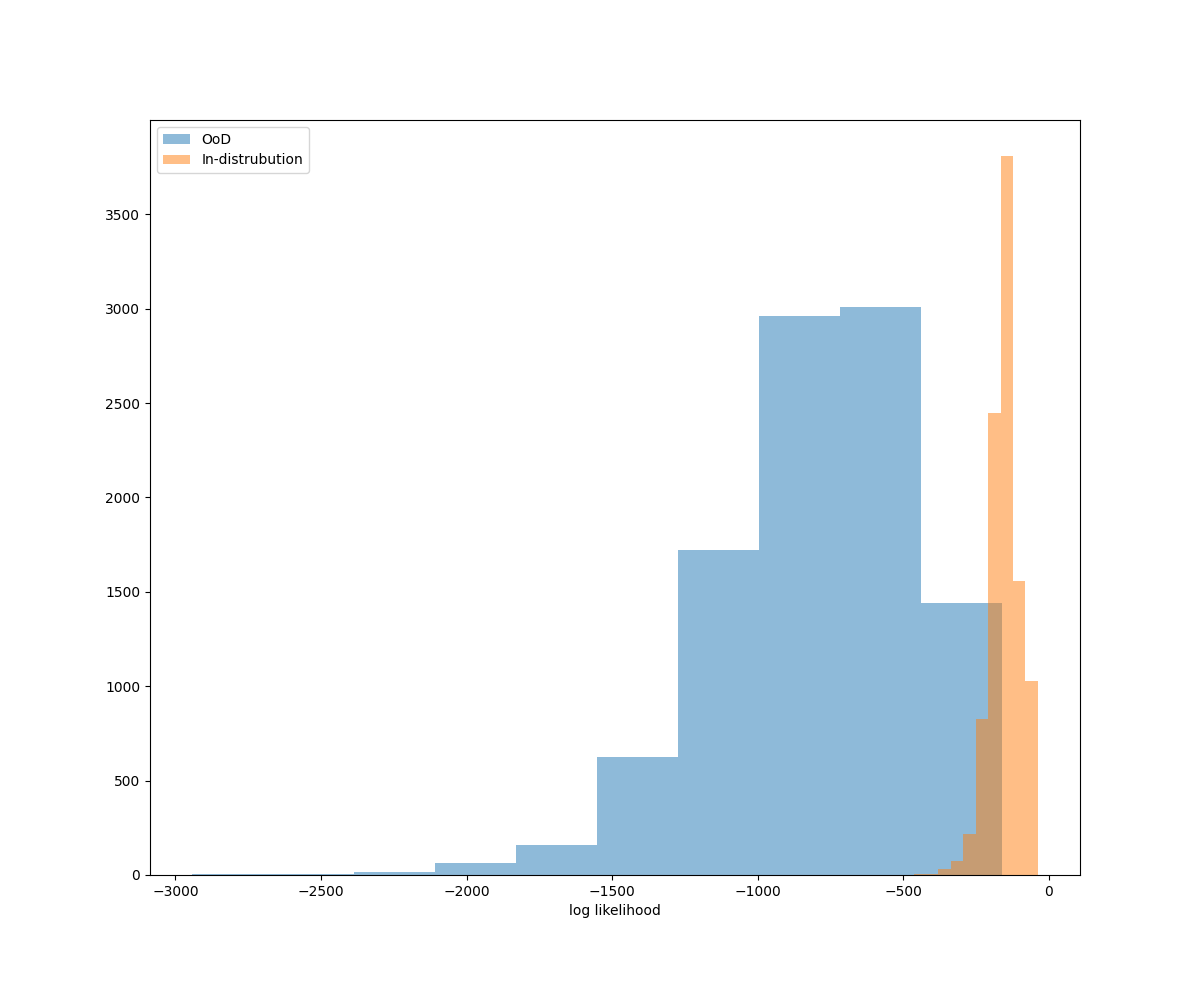
\includegraphics[width=.9\linewidth]{../figures/plot_hist.png}
  \caption{}
  \label{fig:sub1}
\end{subfigure}%
\begin{subfigure}{.5\textwidth}
  \centering
  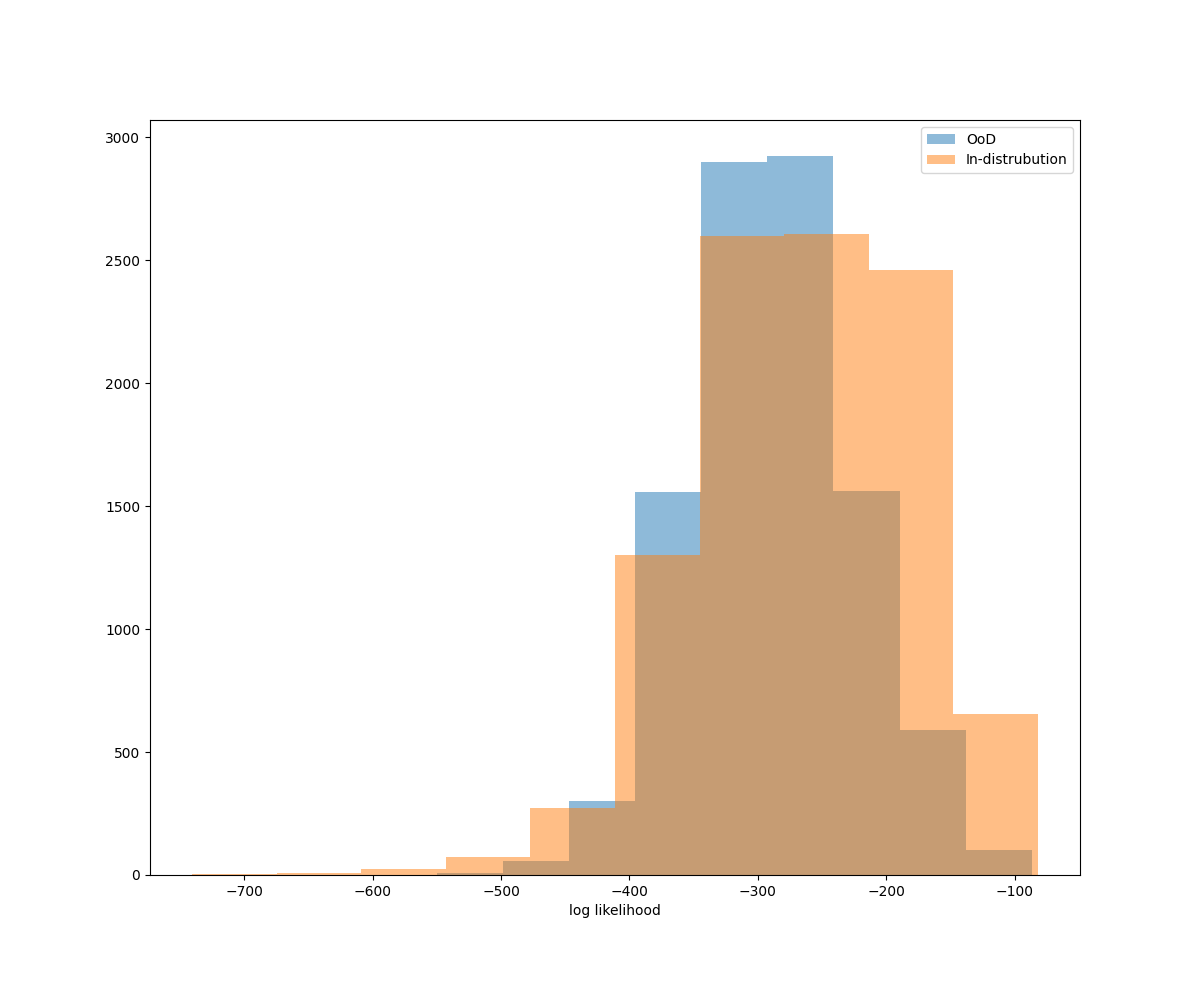
\includegraphics[width=.9\linewidth]{../figures/plot_hist_fmnist.png}
  \caption{}
  \label{fig:sub2}
\end{subfigure}
\caption{Histogram of the log likelihood of test samples for (a) VAE traind on Mnist and Fashion-Mnist as OoD, and (b) VAE traind on Fashion-Mnist and Mnist as OoD}
\label{fig:test}
\end{figure}




\subsection{Metrics}
To classifie whether a data is OoD or not we compute maximum likelihood and then compare with a threshold. The choice of a threshold depends on the particular application. We have tune the threshold, as same as other model hyper parameters, by validation set. 





\mbox{}
\vfill
%\newpage
\bibliographystyle{unsrt}
\bibliography{references}
\end{document}
